\chapter{Background}\label{chap:background} \minitoc

\section{Stream processing as a superset of batch processing} \label{sec:stream-superset}

Batch processing is the processing of data grouped by batches. A batch is a collection of data points that have been grouped by certain criteria. Examples of such criteria could be \textit{"all the transactions from the past two months"}, \textit{"the last million transactions"} or even \textit{"all the transactions made by an user"}. Batch data sets are known as static data \cite{Martin-Batch-Defin}. An example application of such a technique would be processing all the keywords searched for in the google search engine. For instance, grouping the results by keyword and counting how many times a keyword was searched for trend analysis purposes. Batch processing is the oldest paradigm between batch and stream processing. Historically speaking, Apache Hadoop \cite{hadoop} was one of the first widely known technologies for large-scale batch processing, created in 2005. Nearly a decade later, Apache Spark \cite{spark} was released. Spark is capable of doing not only on-disk processing like Hadoop but also in-memory processing, achieving lower processing times. As more and more data became available, the need for stream processing increased. Stream processing refers to the processing of data streams. A data stream is essentially an unbounded data set. This is in contrast to batch processing which works on a finite data set. This distinction is important since some computations are impossible to compute accurately on unbounded data sets. Such an example of an impossible computation on an infinite data set is grouping incoming data by an ID and counting distinct elements.

In order to provide a streaming solution, Apache Spark created the Spark Streaming module. Being a batch system in its core, Spark implements streaming as micro-batching. This approach handles streaming data by grouping incoming events into very small batches. Then, in order to process the entire defined window of data, it joins all micro-batches into a larger one and performs the desired computations. However, this creates an artificial barrier that does not really exist in the streaming context. More than conceptually different from a true stream processing system, processing a stream in a batch fashion, even if in small ones, presents some issues. First, since we are indeed working with batches, results will never be real-time updated per event. For example, if we use a batch size of 100 events, the system would only produce accurate results every 100 events. To handle system inactivity usually these micro-batch systems also have the notion of updating the aggregations with incomplete batches, if no event has entered the system after a pre-specified time period has elapsed. As such, micro-batching was created as a natural implementation of stream processing using the available batch processing systems of the time, but can not be considered true stream processing.

% streaming as a proper superset of batch
Distinguishing between batch and stream processing is important to understand how a monitoring system on top of the latter would work. The Venn diagram \ref{fig:stream-superset} was taken from \cite{batch-is-a-special-case-of-streaming} and illustrates the relation of both processing techniques. A data stream is unbounded or infinite while a bounded data stream has a beginning and an end. Using these definitions, the content of an unbounded data stream contains that of a bounded data set. That is, from an infinite stream, it is possible to fix a left and right boundary in order to obtain a bounded and finite data set. This relation is visible in the \ref{fig:unbounded-bounded-superset} diagram from \cite{batch-is-a-special-case-of-streaming}.

\begin{figure}[!htb]
    \begin{center}
      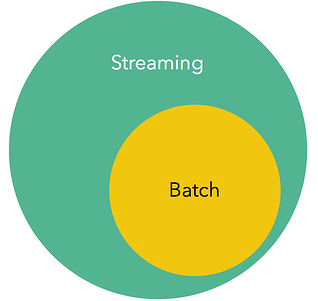
\includegraphics[scale=0.7]{figures/streaming-subset-batch.png}
      \caption{Stream processing as a superset of batch processing}
      \label{fig:stream-superset}
    \end{center}
\end{figure}

\begin{figure}[!htb]
    \begin{center}
      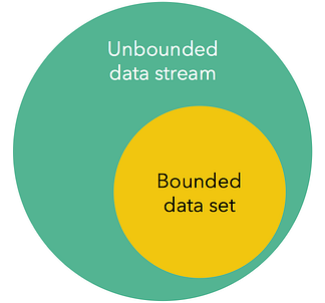
\includegraphics[scale=0.7]{figures/unbounded-superset-bounded.png}
      \caption{Unbounded data streams as a superset of bounded data sets}
      \label{fig:unbounded-bounded-superset}
    \end{center}
\end{figure}


In Section 2.2 we will cover exactly how an unbounded data set (also known as a data stream) can be converted into a bounded data set with the use of windows.


%\section{Anatomy of data analytics}
% data stream is composed by, that may exist or not
%window
%aggregation
%group_by

\section{From unbounded streams to finite data sets} \label{sec:windows}

In Section 2.1 we have defined a data stream as an unbounded data set. But what exactly are the issues of working with an infinite stream of data? Why might we need to convert it into a bounded data set and how to do so? In this Section, we will analyze such issues and present streaming windows as the solution.

% boundless aggregations no need for windows
Computations over an unbounded data set are not impossible. For example, computing the \textit{average} of an event's field for all incoming events is computationally feasible. However, is this boundless average over the stream of events useful? While in some scenarios it may be, more often than not we would like to introduce some logical context into our computations. For instance, consider the monitoring of machines spread out across multiple racks in a large data center. Assume that temperatures measured across all racks are sent to a monitoring system in the form of a data stream. Is the average of all temperatures of all machines over an infinite period useful for the detection of overheating equipment? In this scenario, an average of the temperatures per rack and for the last 5 minutes allows for actionable context, in this case identifying a likely-to-fail rack. To obtain such insight requires computing the average over the last 5 minutes' worth of data, effectively defining a begin and end. By creating such a conceptual range, we realize that in practice we need a bounded data set. Partitioning an infinite data stream to obtain such a finite data set is made through the use of windows.

The authors of \cite{Wang-Windows-Stream-Processing} claim that \textit{"recent history is often managed using windows"} and that \textit{"windowing makes it possible to implement streaming versions of the traditionally blocking relational operators, such as streaming aggregations"}. More formally, the authors of \cite{Botan-SECRET} state that \textit{"a window W over a stream S is a finite subset of S"}.

% 2 dimensions of windows
Windows can be categorized by two dimensions: the window size \textit{W} and the sliding step size \textit{S}, both either tuple or time-based. Tuple-based windows' size is specified by the number of items the window can contain and time-based windows specify the time interval worth of incoming data a window can store. For instance, a tuple-based window of size $10^3$ tuples will store exactly $10^3$ items. In contrast, a time-based window storing the last 5 minutes of events can contain a varying number of tuples but will always keep the events arrived in the last 5 minutes. A window slides over incoming data and groups it, enabling us to compute aggregations over a defined and bounded set of events. The step size \textit{S} of a windowing technique is formally defined by \cite{Botan-SECRET} as \textit{"the distance between consecutive windows"}. This means that two consecutive windows W\textsubscript{1} and W\textsubscript{2} are exactly \textit{S} units away. As mentioned, these units can be units of time or a number of tuples.

There are three types of windows: true sliding, stepping or tumbling windows.
% true sliding: unitary steps
A true sliding window is defined by any given window size \textit{W} and a unitary step (\textit{S}=1), which can be defined as time or tuple-based. At each step, the window advances one unit, which may be one event for tuple-based steps, or one time-unit whether that is in milliseconds, seconds, days, weeks or another magnitude of time, measured based on the system clock or event time. Such a true sliding movement can be observed in Figure \ref{fig:sliding-window} with a tuple-based window of size \textit{W} of three tuples and unitary step. 

\begin{figure}[!htb]
    \begin{center}
      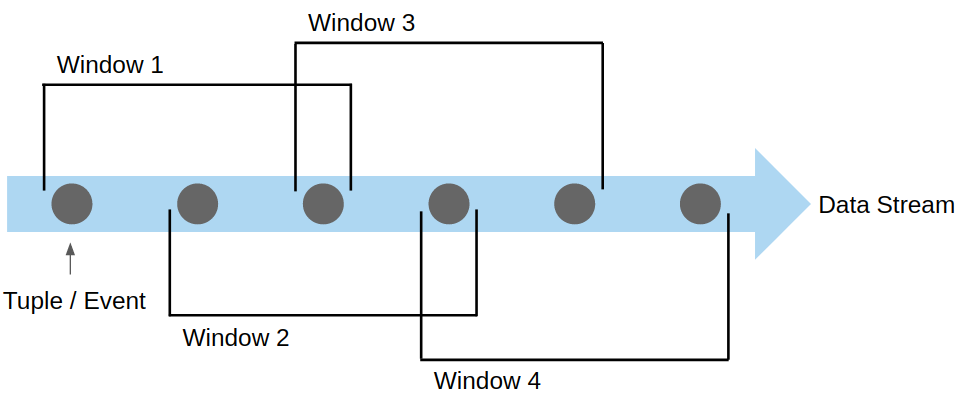
\includegraphics[scale=0.3]{figures/sliding.png}
      \caption[True sliding window]{True sliding window, W=3, S=1}
      \label{fig:sliding-window}
    \end{center}
\end{figure}

% stepping windows (per x units over Y window size)
% stepping: step > 1 < window size
A stepping window behaves exactly like a true sliding one but the step size \textit{S} is not unitary. In other words, a stepping window is defined by any window size \textit{W} and steps \textit{S} greater than a unit. Once again, both the window and step sizes, \textit{W} and \textit{S} respectively, can be time or tuple-based. Figure \ref{fig:stepping-window} represents a stepping tuple-based window of size \textit{W} of three and a stepping size \textit{S} of two.

\begin{figure}[!htb]
    \begin{center}
      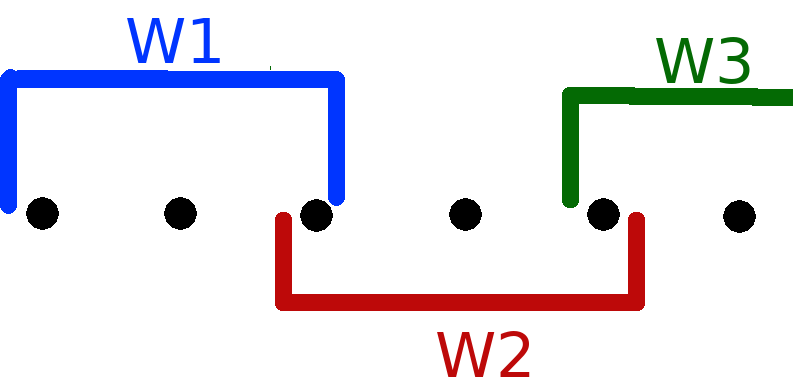
\includegraphics[scale=0.3]{figures/stepping.png}
      \caption[Stepping window]{Stepping window, W=3, S=2}
      \label{fig:stepping-window}
    \end{center}
\end{figure}

% tumbling: step = window size
A tumbling window, also defined by its window size \textit{W} and step size \textit{S}, is a window where W is equal to S. Hence, tumbling windows partition the stream into non-overlapping chunks with the same size. Since the intersection of different tumbling windows is always empty, each event is said to belong to exactly one tumbling window. An example of a tumbling window can be seen in Figure \ref{fig:tumbling-window} with a tuple-based window of size \textit{W} of three and an equally large step size \textit{S}.

\begin{figure}[!htb]
    \begin{center}
      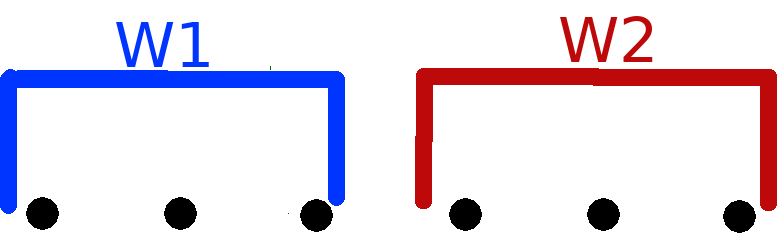
\includegraphics[scale=0.3]{figures/tumbling.png}
      \caption[Tumbling window]{Tumbling window, W=S=3}
      \label{fig:tumbling-window}
    \end{center}
\end{figure}

The mathematical expression below summarizes our categorization of sliding windows.
\begin{equation} 
  Window \,\, of \,\, size \,\, W, \,\, step \,\, S =
    \begin{cases}
      true \,\, sliding & \text{if \textit{S}=1}\\
      stepping & \text{if \textit{S}>1}\\
      tumbling & \text{if \textit{S}=\textit{W}}
    \end{cases}
\end{equation}

For the scope of this Thesis, we will work under a time-based sliding window framework with a unitary step size. Despite focusing on time-based true sliding windows, our approach is just as valid for tuple sized windows and for other step values as well.

\section{Aggregations over data streams} \label{sec:aggregations}

An aggregation --- also known as a fold, reduce or accumulate --- is an operation that reduces a collection of values to a single one. Examples of such are the computation of data set sums, minima, averages or the number of distinct elements (cardinality). An aggregation may be exact or approximate. Exact aggregations compute a value from a sequence of elements, where no error or loss of resolution exists. On the other hand, approximate aggregations have an error margin to the associated aggregation value which is usually controllable by adjusting a set of parameters. Approximate aggregations trade precision of results for efficient time and space usage. Such trade-off between accuracy and time/space efficiency will be made clear when discussing some of the existing approximate aggregators in Section \ref{sec:pds}.

Aggregations are present in most programming languages and frameworks. Quoting from the JavaSE13 documentation on the \textit{Stream.reduce()} method\footnote{https://docs.oracle.com/en/java/javase/13/docs/api/java.base/java/util/stream/package-summary.html\#Reduction}: \textit{"A reduction operation (also called a fold) takes a sequence of input elements and combines them into a single summary result by repeated application of a combining operation"}. Hadoop's MapReduce paradigm consists of first applying \textit{map} steps to the collection of data and then a \textit{reduce} one. \textit{Map} tasks will transform each item as desired and the \textit{reduce} task will merge the collection into a single value. Reduce methods make use of a \textit{combine} function and recursively apply it. The \textit{combine} function takes the current aggregation value and combines it with the next item in the set, returning the new aggregated state. Doing this recursively for each item in the collection results in a single value: the aggregate value for the data set.

\subsection{Aggregation properties}
\label{sec:agg-properties}

Different aggregations have different properties. These properties are listed in \cite{Tangwongsan-Sliding-Window-Aggregation-Algorithms}, where the authors group different aggregations according to the properties they satisfy. Table \ref{tbl:aggregations-properties} was adapted from this work and categorizes different families of operations based on said properties.

\begin{table}[!htb]
    \begin{center}
      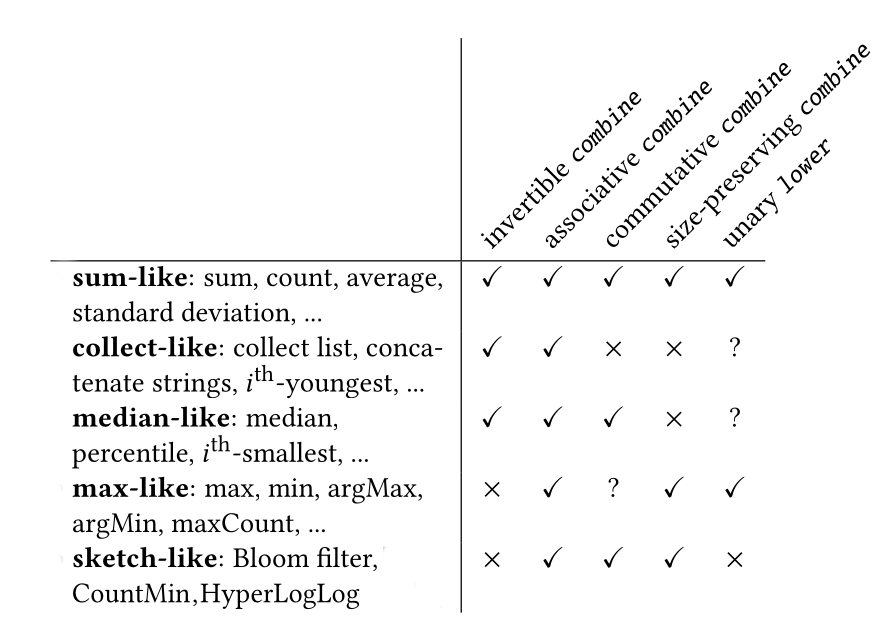
\includegraphics[scale=0.5]{figures/aggregation-operations-properties.png}
      \caption[Aggregation properties]{Aggregation properties. Checkmarks (\checkmark), crosses ($\times$), and question marks (?) indicate a property is true for all, false for all, or false for some of a given group of like operations, respectively}
      \label{tbl:aggregations-properties}
    \end{center}
\end{table}

To understand these properties, we must be familiar with the \textit{combine} and \textit{lower} functions. The already mentioned \textit{combine} function merges the incoming event with the incrementally computed aggregation state. The \textit{lower} function is responsible for returning a result for a given query according to the current aggregation state. For instance, consider the use case of computing a sum aggregation over a window of data. The \textit{combine} function would be the arithmetic operator \textit{+} and would merge the current aggregation state --- \textit{i.e.} the current sum value --- with the new incoming event. The \textit{lower} function would return the current aggregation state --- \textit{i.e.} return the total sum computed.

The following are formal definitions of these properties and were summarized from \cite{Tangwongsan-Sliding-Window-Aggregation-Algorithms}. An aggregation operation is said to have:

\begin{enumerate}
    \item  an \textbf{\textit{invertible combine}} if a function $\ominus$ exists such that $(x \oplus y) \ominus y = x$, for all $x$ and $y$
    
    \item  an \textbf{\textit{associative combine}} if $(x \oplus y) \oplus z = x \oplus (y \oplus z)$, for all $x$ and $y$
    
    \item  a \textbf{\textit{commutative combine}} if $x \oplus y = y \oplus x$, for all $x$ and $y$
    
    \item  a \textbf{\textit{size-preserving combine}} if the aggregation state resulting from $\oplus$ always occupies the same space in memory
   
    \item  a \textbf{\textit{unary lower}} if the query does not need any parameters --- \textit{e.g.} a membership test with a Bloom filter would require the element to test membership for as a parameter so it is not unary; returning the total sum is unary since it does not require any parameters
\end{enumerate}

%These properties are used to evaluate SWAG algorithms. Different algorithms might only apply to certain families of aggregations. This way, the multiple SWAG algorithms presented throughout this Thesis will be analyzed not only on their time and space complexity but also on the restrictions they impose regarding the aggregation' properties required.

\subsection{Sliding Window Aggregations}

Unlike many other scenarios that focus on data at rest, streaming aggregations handle data in motion. While some aggregations can be computed on an infinite data set, often we want to compute these over a finite one. As we have seen in Section \ref{sec:windows}, to obtain a bounded data set from a data stream we apply windowing techniques. In doing so, we obtain a finite data set denoted as a sliding window and compute aggregations over it. The authors of \cite{Tangwongsan-Sliding-Window-Aggregation-Algorithms} define such aggregations over sliding windows as Sliding Window Aggregations (SWAGs). Once again let us consider the data center temperature monitoring problem from Section \ref{sec:windows} as an example use-case for SWAGs. How would we compute the average temperature per rack in the data center in the last 5 minutes? To better understand, let us translate this question to a streaming SQL query, with a similar syntax to the API provided by Apache Flink \cite{flink}. Assuming all the temperatures can be queried from the \textit{Temperatures} table and that each rack corresponds a different \textit{rack\_id} we have the following query:

\begin{verbatim}
SELECT rack_id, AVG(temperature)
FROM Temperatures
GROUP BY TUMBLE(timestamp, Time.minutes(5), rack_id)
\end{verbatim}

In the query above, the \textit{TUMBLE(timestamp, Time.minutes(5), rack\_id)} statement groups incoming data using time-based tumbling windows of 5 minutes duration, using the \textit{timestamp} field to evict events not in this time interval. The resulting list of rows has \textit{rack\_id} as its key and as corresponding value a list of temperatures, from the past 5 minutes. Finally, for each rack and its list of temperatures, we compute an \textit{AVG} aggregation, resulting in the average temperature per rack in the past 5 minutes.


\subsection{Sliding Window Aggregation Algorithms} \label{sec:back-swag-algs}

A sliding window aggregation (SWAG) algorithm allows the computation of an exact or approximate aggregation over a sliding window. A SWAG algorithm may restrict the set of possible to compute aggregations based on their properties. Different SWAG algorithms use different data structures for the window contents and the incremental aggregation state.

The aggregation properties analyzed in Section \ref{sec:agg-properties} are used to evaluate SWAG algorithms. Different algorithms might only apply to certain families of aggregations. This way, the multiple SWAG algorithms presented throughout this Thesis will be analyzed not only on their time and space complexity but also on the restrictions they impose regarding the aggregation' properties required.

Tangwongsan et al. present two of the most basic SWAG algorithms: \textit{Recalculate From Scratch (RFS)} and \textit{Subtract On Evict (SOE)}.

\subsubsection{Recalculate From Scratch}
Recalculate From Scratch (RFS) is the simplest and most general SWAG algorithm. As the name suggests, this algorithm recomputes the aggregation over the entire window for each insertion and eviction. For instance, the computation of a sum over a sliding window using RFS means that upon each insertion or eviction all elements are summed.

This approach does not restrain the aggregation in terms of properties: it works for every family of aggregations. However, given \textit{n} as the window size, this algorithm takes \textit{O(n)} space and time complexity which makes it unfit in most scenarios of large scale data processing. 

\subsubsection{Subtract On Evict}
Subtract On Evict (SOE) only works for aggregations whose  \textit{combine} $\oplus$ function is invertible. That is, as defined in Table \ref{tbl:aggregations-properties}, a function $\ominus$ exists such that $(x \oplus y) \ominus y = x$.

SOE inserts new elements into the window and combines the previous aggregation value with the new element. On eviction, SOE applies the inverse of the combine function, $\ominus$, to expire the evicted element from the aggregation state.

With window size of \textit{n}, SOE has \textit{O(n)} space complexity and \textit{O(1)} time complexity. However, aggregations are not always invertible thus making this algorithm very restrictive and not always applicable.


% \section{Concept drift}
% seasonal and evolutionary
% static ML models
% data pattern shifts -> in this context, concept drift
% data pattern shifts can be formally defined and introduced as concept drift IN THIS PARTICULAR CASE of monitoring a stream that feeds into ML models